\section{Introduction} \label{sec:intro}

% The introduction contains clear statement of the project, the current situation about the work on the project, the scope of the report, organization of the report. 

% ========== Problem statement ========= %

The growing cat population keeps making it more and more challenging for humans to take care of them. There are hundreds of cats living in large territories like campuses, sanctuaries and more so in the streets. Even if some cats are taken under our wings to look after at our homes it might be challenging to follow their dietary behaviours. In regards to the immensely fast developing technology, there seems to be very little improvement and innovation when it comes to cat feeding systems. The already existing systems are too costly and incapable of tracking cat diets even for a single cat. The state of the art, according to an article on most rated automatic cat feeding systems of 2019 \cite{cite:SOTA}, has several key features. These are large food storage capacity, portion control settings, kibble size options and pet-proofing. This system costs 150 dollars. The absence of advanced monitoring systems leaves cats unsupervised where survival of the weaker cats is less probable. Because of this, it is not possible to detect cats that are in need of an external assistance of food and intervene. Aside from this, the absence of smart, inexpensive systems cause risks for both the cat and human health due to the unsanitary living conditions it creates. Figure~\ref{fig:foodfloor} shows some pictures taken recently at the campus of Middle East Technical University which illustrate the situation at hand effectively. In the era of everything smart and connected it is only logical to propose, design and implement a solution, using novel techniques, which fills the gap in the untapped market of automatic cat feeding systems. Making our, homo sapiens', lives easier while also caring for our companions, Felis Catus, Felerest aims to solve these issues by taking on the challenges at hand while also providing customer oriented additional features.

\begin{figure}[ht]
     \centering
     \begin{subfigure}[b]{0.49\textwidth}
     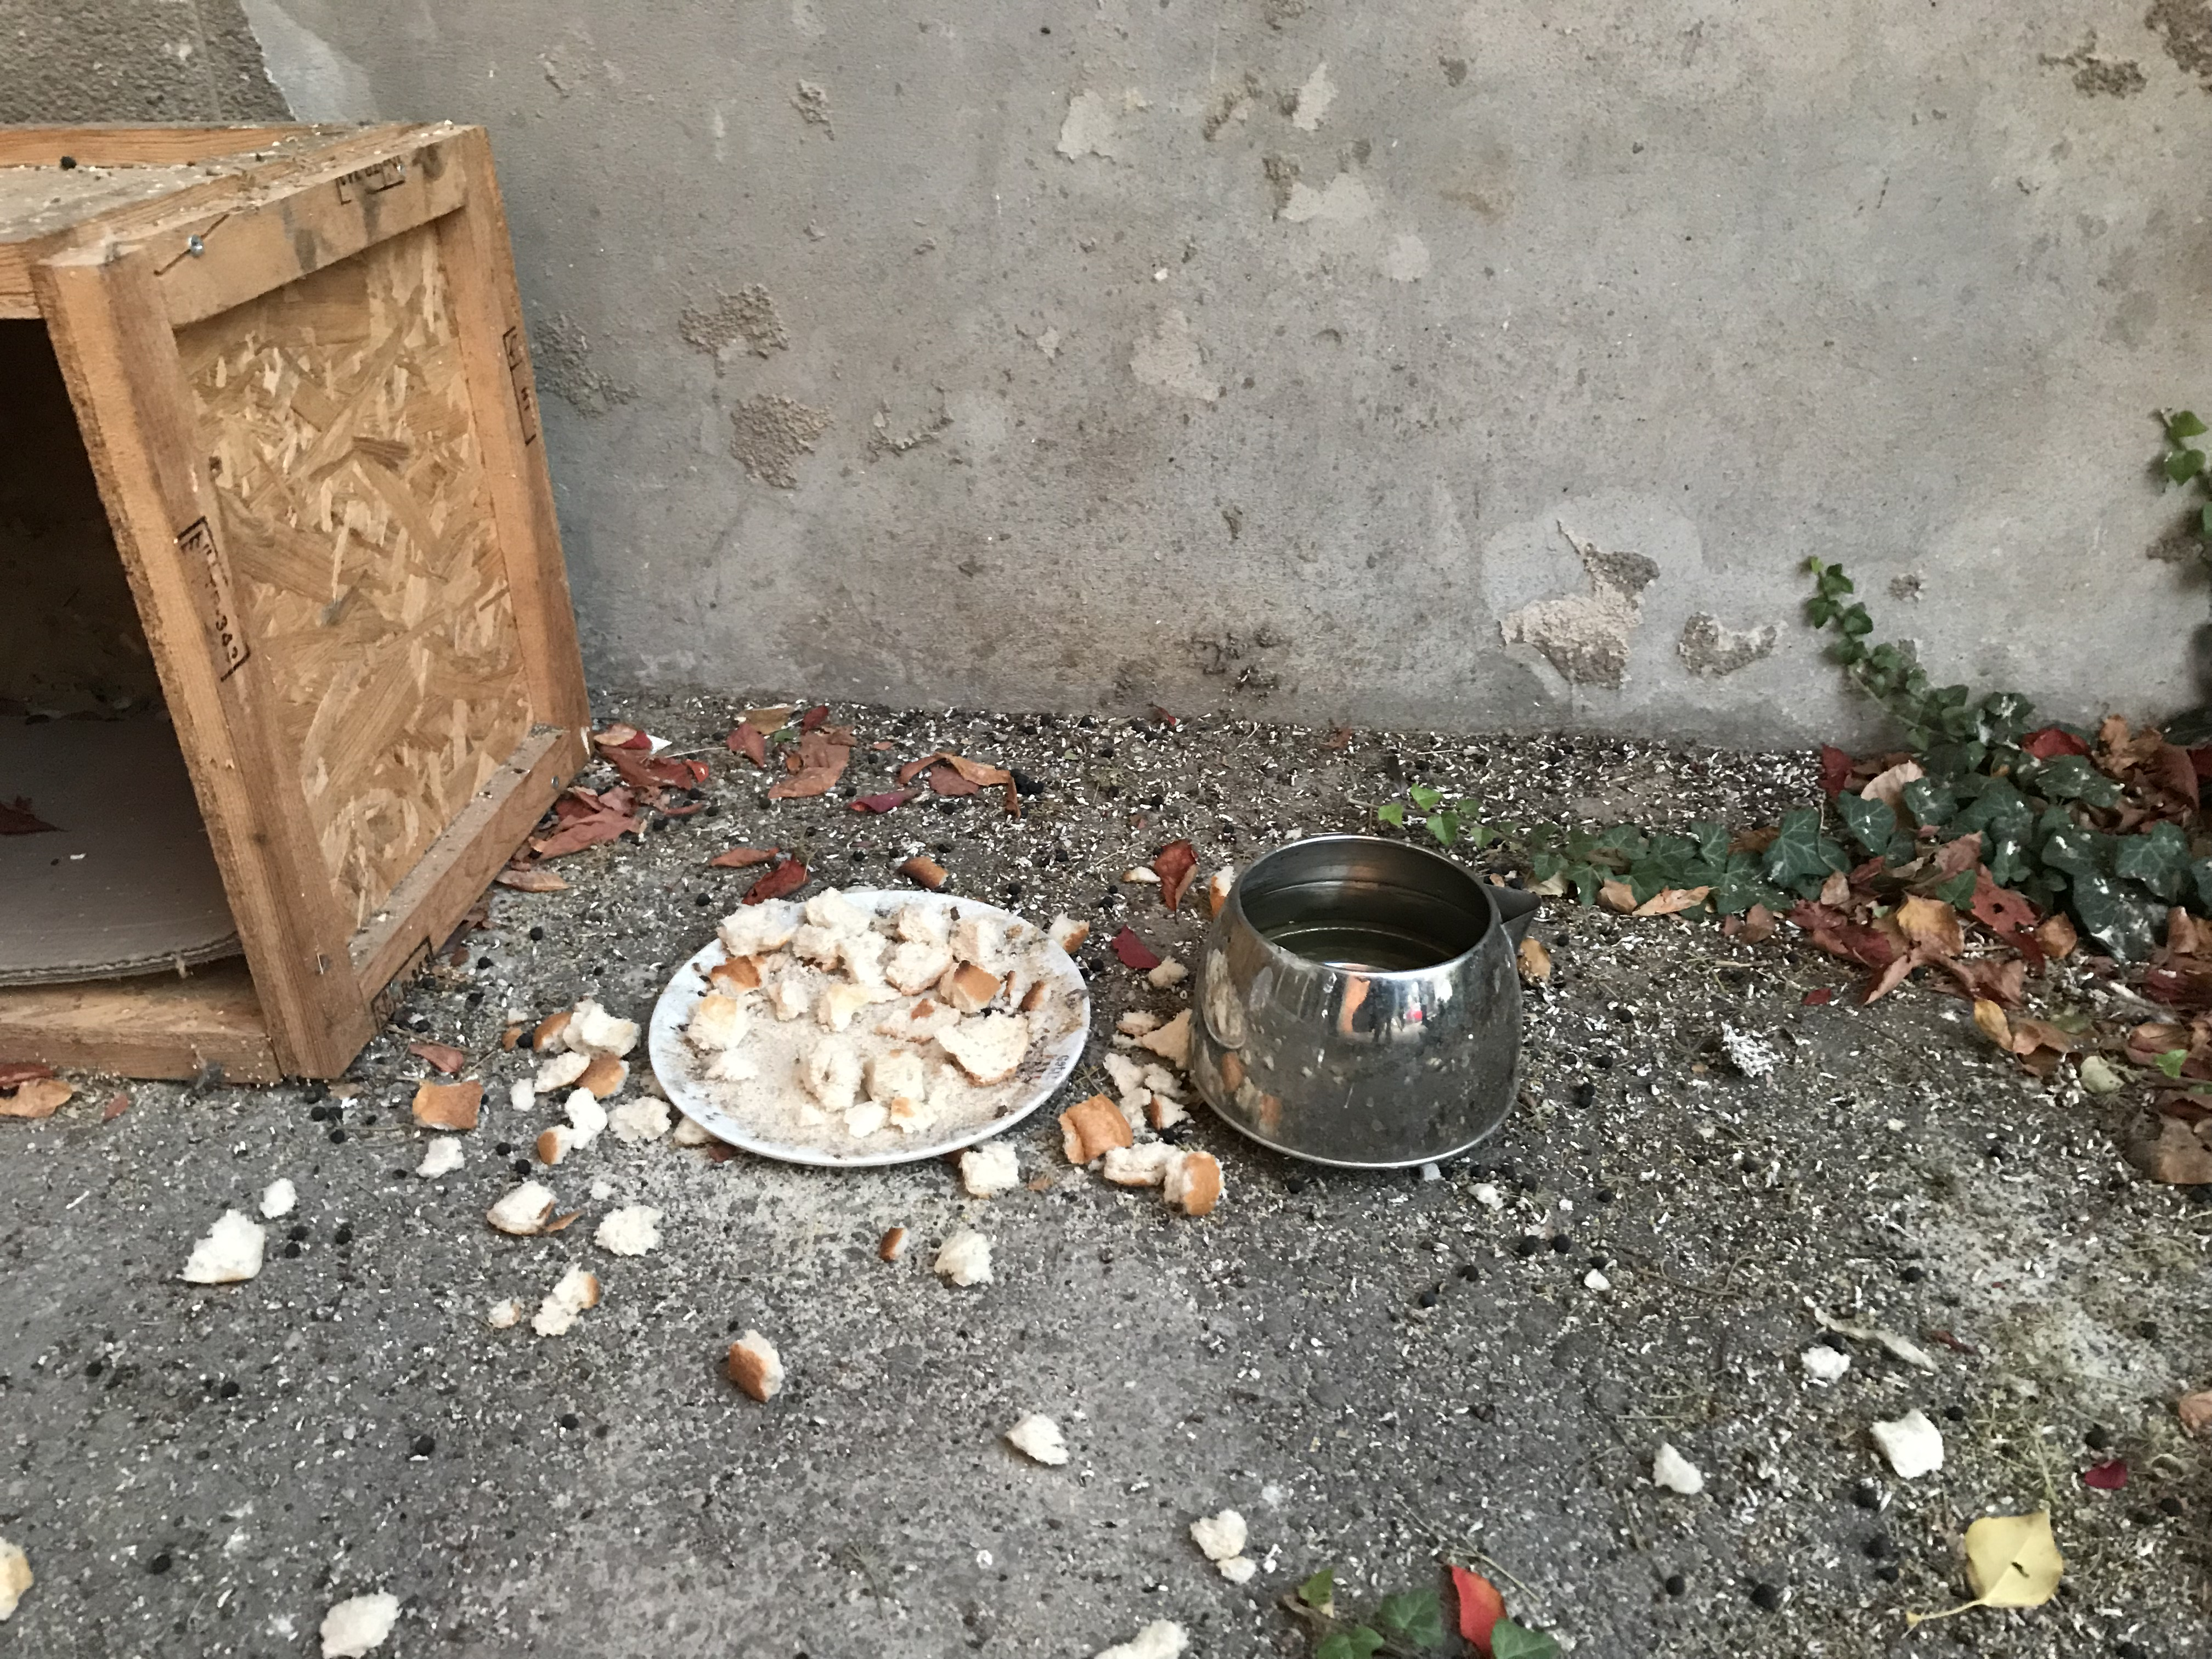
\includegraphics[width=\linewidth]{img/foodfloor1.jpg}
     \caption{}
     \label{fig:foodfloor0}
     \end{subfigure}
     \begin{subfigure}[b]{0.49\textwidth}
     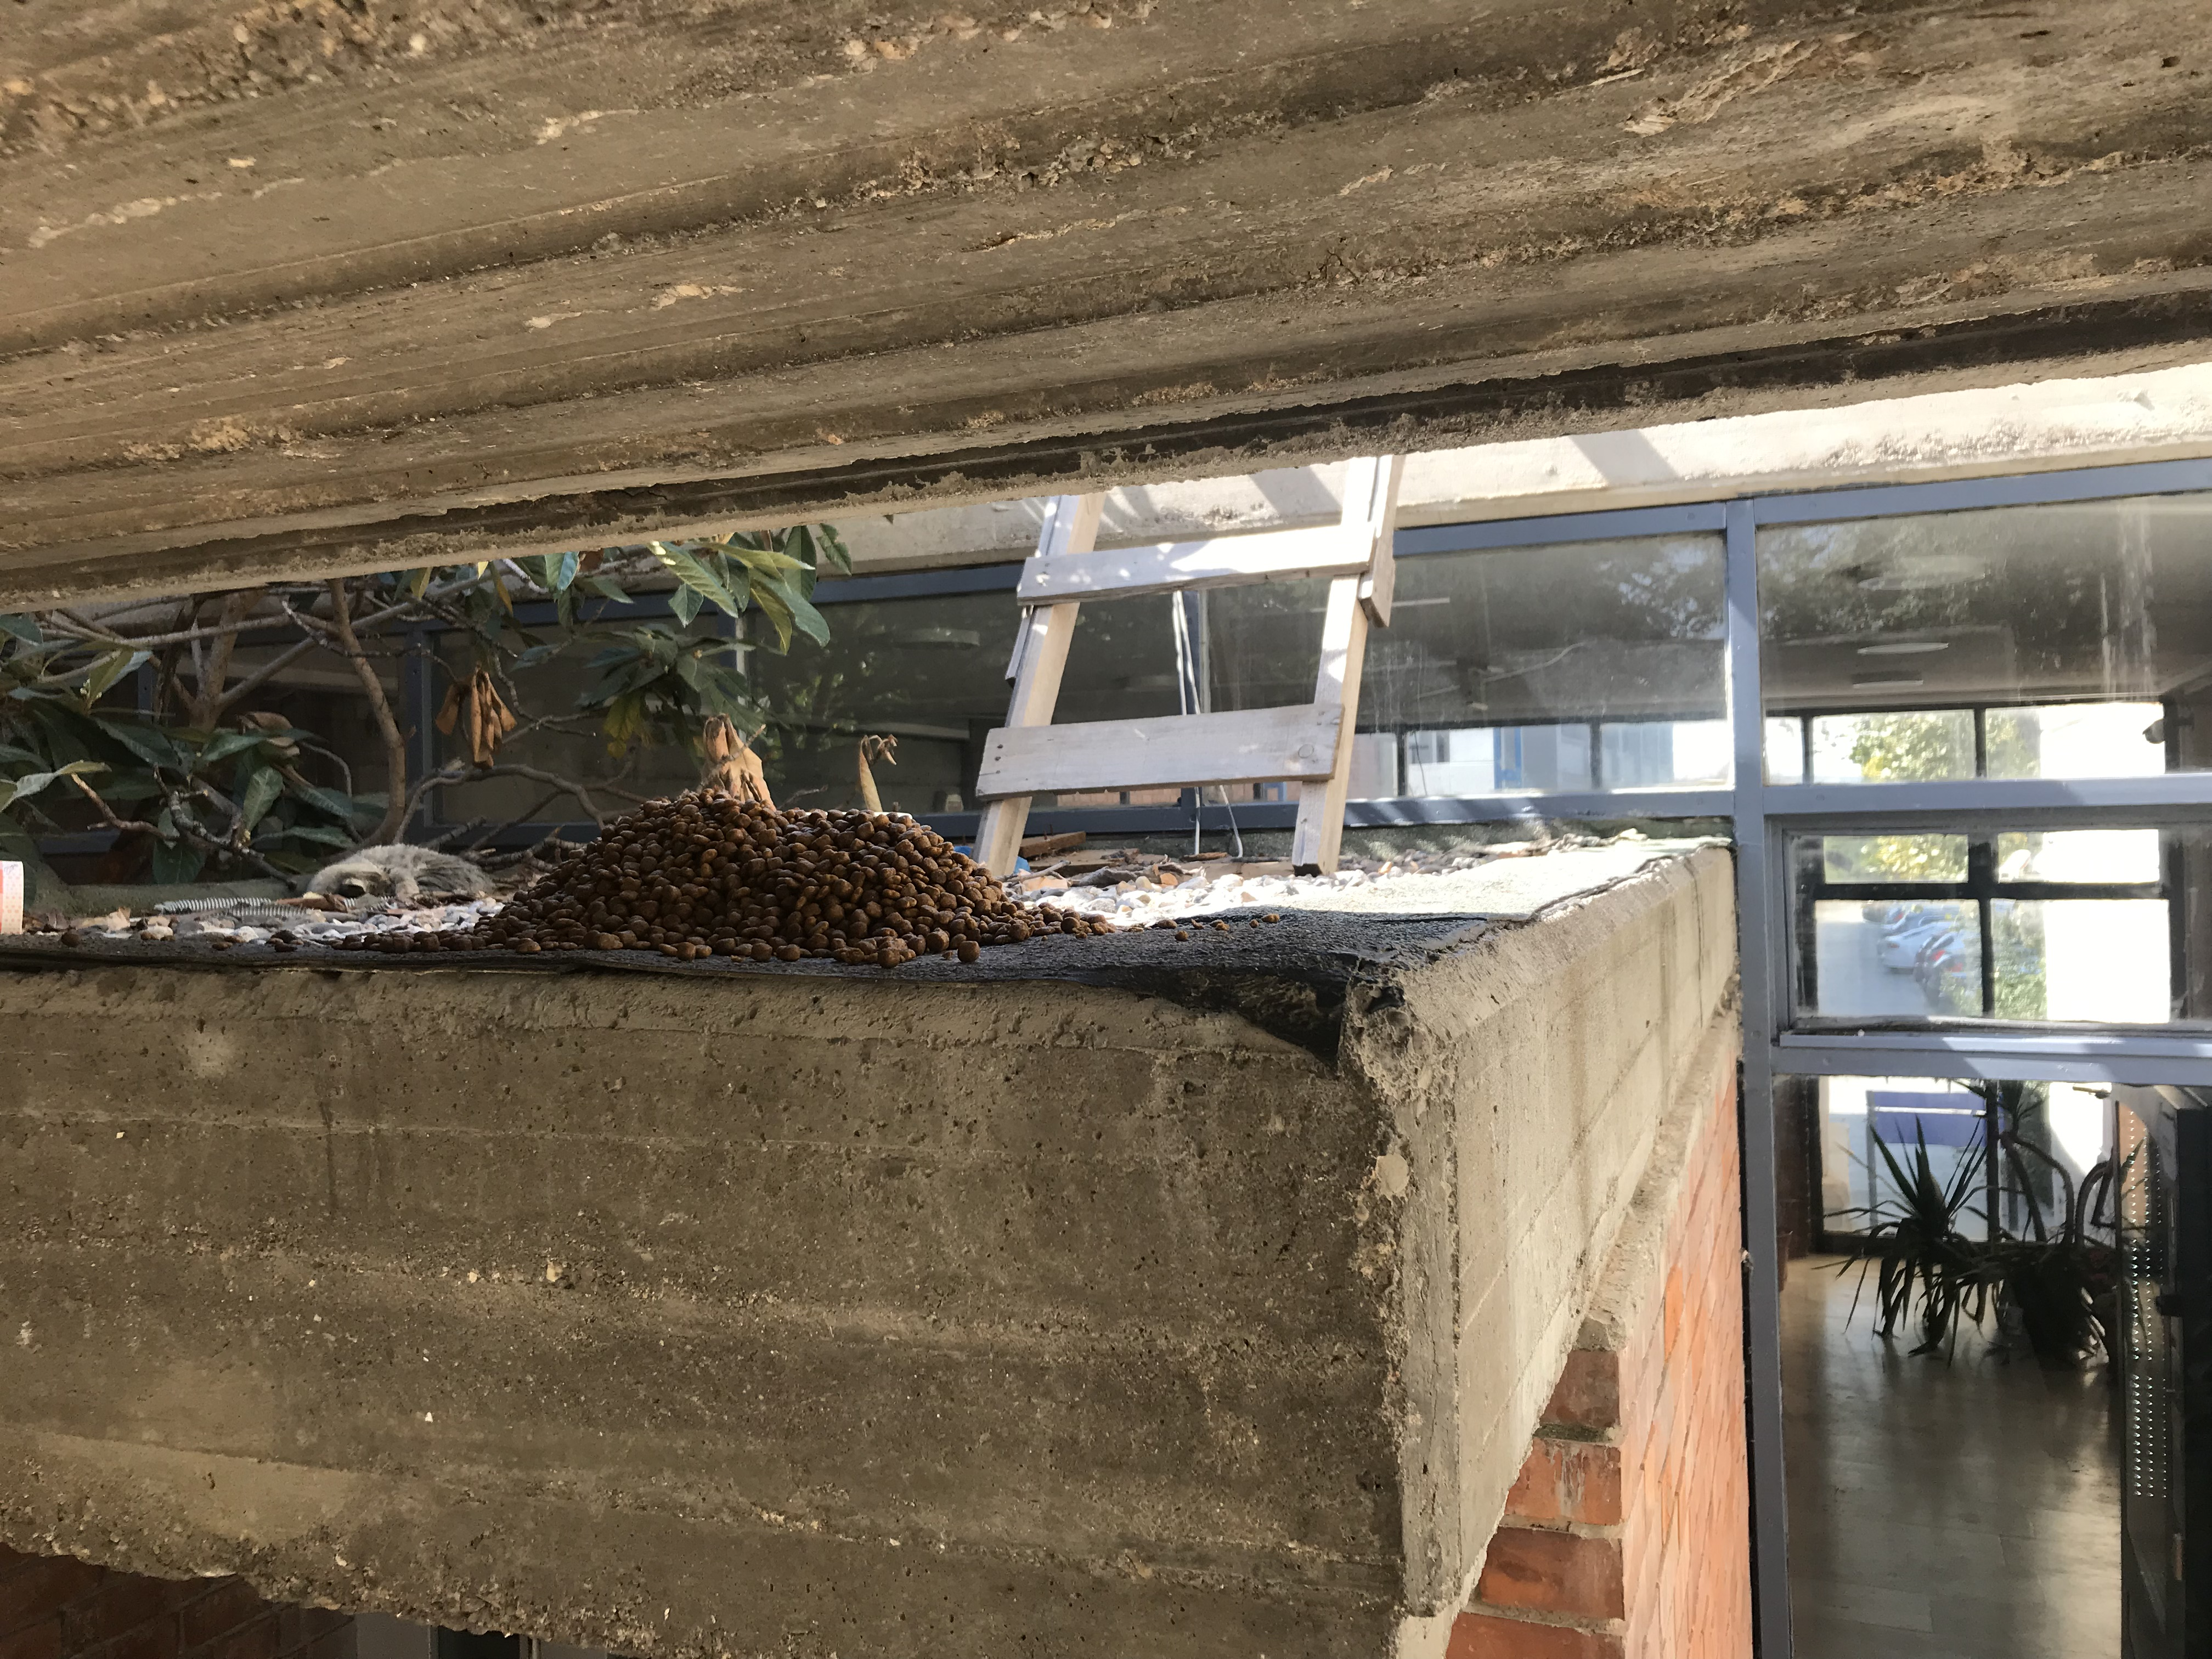
\includegraphics[width=\linewidth]{img/foodfloor2.jpg}
     \caption {}
     \label{fig:foodfloor1}
     \end{subfigure}        
     \caption{Photos from METU's campus}
     \label{fig:foodfloor}
\end{figure}


% ======= Background information ======= %

The motivation behind Felerest's work is to solve the aforementioned problems and bring more to the table. The final product's budget is 200 dollars, the marketing price is foreseen to be less than this which will surely rattle the market in the positive sense. The system will be capable of feeding a large number of cats making it adoptable for usage in campuses and homes where cats are plentiful. The system's reservoir will be adequate to feed more than 20 cats for the duration of the battery lifetime.

The goal is to identify cats and feed them amounts inversely proportional to their weights. This feeding system is achieved automatically by implementing a camera to the box and processing the images obtained from the camera to detect the presence of cats. The food container inside the box releases cat food from a rotating mechanism. The system releases food proportional to the number of cats present with regard to each cats weight, thin cats get more food while thicker cats get less. This system's purpose is to monitor each cats dietary actions individually and feed them accordingly, therefore the optimal usage is defined for cases where cats approach the box one by one. Although not as efficiently, the system is capable of feeding more than a single cat at once. Moreover, the system has the ability to function for a minimum of 5 hours on charged battery life with the additional feature of working as plugged to a power supply. The user will have access to a web interface, which contains information on how much food is left in the container, how many times each individual cat has visited the box, how many new cats were recognized and added to the log, the remaining battery lifetime while also providing images of the cats taken from the camera which will be a way to remotely track the visual of the cats. An extra feature of this system which distinguishes it from all other existing solutions is the dog deterring module. This is the key factor which makes it possible for outside usage. This way cats can safely approach the box without dogs eating their food or scaring them away. 

% ===== Organization of the report ===== %

In this report the subsystems constituting the overall system are identified and explained in detail by investigating each module that forms the subsystem. There are 4 subsystems in total: computer vision, electronics, mechanics, and back-end. The technical and implementation details at a subsystems level constituting the parts of the overall system are fully explained with technical details and supporting visual content. Algorithm details are included for Computer vision and back end parts. Alongside these, the requirements for each subsystem, the proposed solutions, the effectiveness of the solutions and their evaluations, possible foreseen risks and difficulties, testing procedure, testing results and action taken in regard to these results, planned future work in each subsystem and future test plans as a measure of success are investigated in this report. The tests of these subsystems and their results are examined exclusively. To effectively transfer these to the reader, first a general description of the overall system will be provided with solutions that satisfy the necessary requirements. In this part, the expected weight, dimension and the total power consumption of the system will be stated. Afterwards, each subsystem will be explained with its modules as defined earlier. After the subsystems are clear, the integration process and the measure of success will be discussed. A cost analysis of the final product will be explored. The deliverables of the project will be considered. Finally, the analysis of the proposed solutions will be recapped alongside a review about the remarks made throughout the process.  


    